\documentclass[border=4pt]{standalone}
\usepackage{tikz}
\usetikzlibrary{positioning, arrows.meta, shapes.geometric, calc, fit, backgrounds}
\usepackage{amsmath,amssymb}

\begin{document}
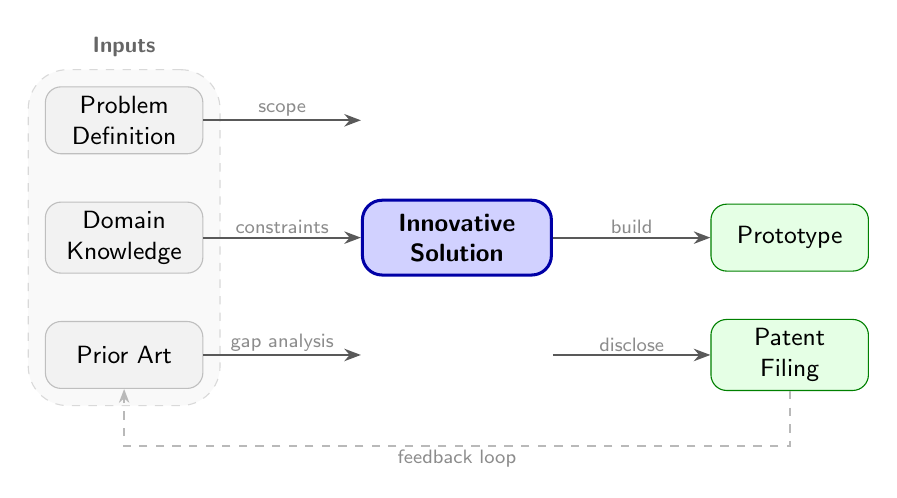
\begin{tikzpicture}[
  input/.style={draw, rounded corners=2mm, minimum width=2.0cm, minimum height=0.85cm,
                fill=gray!10, draw=gray!50, align=center, font=\sffamily\small},
  innov/.style={draw, rounded corners=2.5mm, minimum width=2.4cm, minimum height=0.95cm,
                fill=blue!18, draw=blue!65!black, line width=1.1pt, align=center,
                font=\sffamily\small\bfseries},
  output/.style={draw, rounded corners=2mm, minimum width=2.0cm, minimum height=0.85cm,
                 fill=green!10, draw=green!50!black, align=center, font=\sffamily\small},
  arr/.style={-{Stealth[length=6pt]}, thick, color=black!65},
  arrd/.style={-{Stealth[length=5pt]}, dashed, color=gray!55, thick},
  lbl/.style={font=\sffamily\scriptsize, text=black!45, fill=white, inner sep=1pt},
  glbl/.style={font=\sffamily\footnotesize\bfseries, text=black!60}
]

  % Input nodes
  \node[input] (in1) {Problem\\Definition};
  \node[input, below=0.6cm of in1] (in2) {Domain\\Knowledge};
  \node[input, below=0.6cm of in2] (in3) {Prior Art};

  % Innovation node
  \node[innov, right=2.0cm of in2] (core) {Innovative\\Solution};

  % Output nodes
  \node[output, right=2.0cm of core] (out1) {Prototype};
  \node[output, below=0.6cm of out1] (out2) {Patent\\Filing};

  % Arrows from inputs to core
  \draw[arr] (in1.east) -- (core.west |- in1.east) node[lbl, midway, above] {scope};
  \draw[arr] (in2.east) -- (core.west) node[lbl, midway, above] {constraints};
  \draw[arr] (in3.east) -- (core.west |- in3.east) node[lbl, midway, above] {gap analysis};

  % Arrows from core to outputs
  \draw[arr] (core.east) -- (out1.west) node[lbl, midway, above] {build};
  \draw[arr] (core.east |- out2.west) -- (out2.west) node[lbl, midway, above] {disclose};

  % Feedback arrow
  \draw[arrd] (out2.south) -- ++(0,-0.7) -| (in3.south) node[lbl, pos=0.25, below] {feedback loop};

  % Background group around inputs
  \begin{scope}[on background layer]
    \node[fit=(in1)(in2)(in3), draw=gray!30, dashed, rounded corners=5mm,
          inner sep=6pt, fill=gray!5] (ginput) {};
    \node[glbl, above=1pt of ginput.north] {Inputs};
  \end{scope}

\end{tikzpicture}
\end{document}